\section{Evaluation}\label{sec:evaluation}

In this part, we evaluate the performance of our solution via simulation.

\textbf{Network topology and routing function}: the network topology we use for our simulation is a n-hop cycle. We randomly generate k paths of various lengths (varies from 2 to n-1) to traverse  the cycle. These k paths are divided into two sets $R_{old}$ and $R_{new}$. Our simulator ensures that  $R_{old} \cup R_{new}$ introduces cyclic buffer dependency. The using of a cycle as the network topology is representative for our purpose because only the paths
traversing some cycle in the network are related to cyclic buffer dependency. 

 %The using of a cycle as the network topology is representative for our purpose because the routing reconfiguration of the part of paths not traversing any cycle in a DCN is not related to any potential cyclic buffer dependency. 
 
 %Further, although the topology of DCNs could contain multiple cycles, the routing reconfiguration of paths in different cycles are independent in terms of calculating some configuration depdendencies for avoiding cyclic buffer dependency.

\textbf{Compared scheme}: In our simulation, we compare our solution with the naive two-stage solution, i.e., removing all the paths in $R_{old}$ in the first stage, and adding the paths in $R_{new}$ in the second stage.

\textbf{Configuration time of a single path}: In our simulation, we simply assume the time cost to configure a path is equal to the number of switches this path traverses in the network. The study of a more realistic model for estimating the time cost of configurating a path is left as a future work.

\begin{figure}[t]
	\centering
	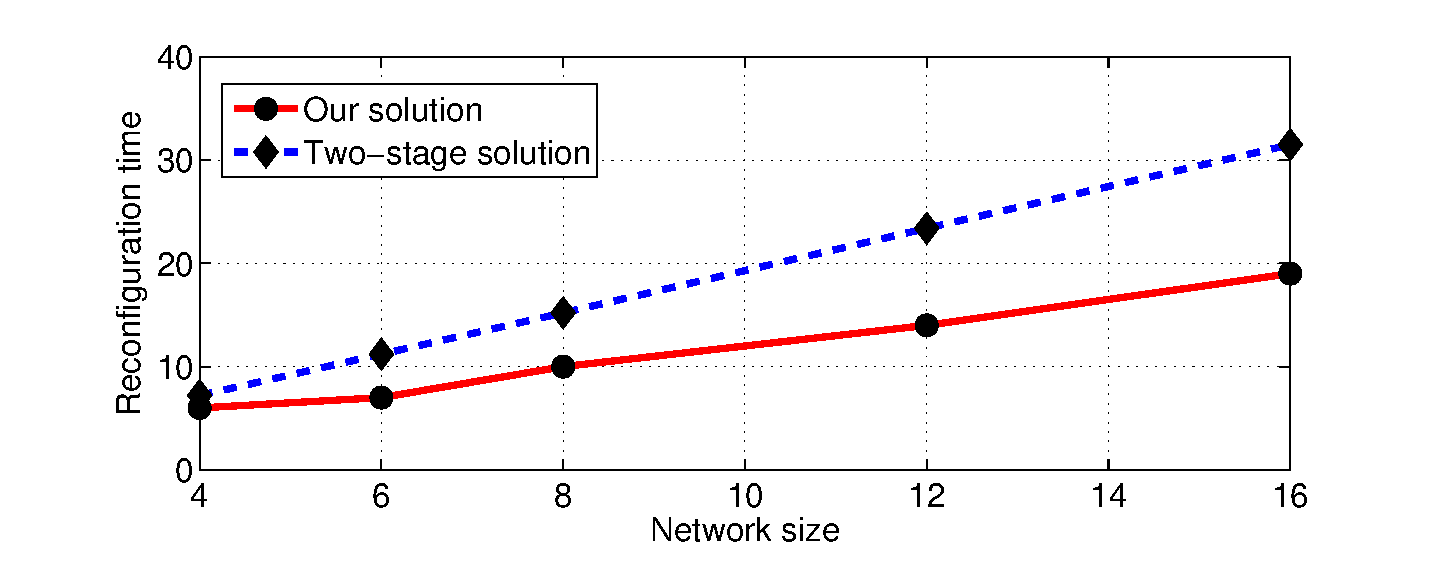
\includegraphics[width=0.45\textwidth] {figs/conftime.eps}
	\caption{Routing reconfiguration time under two solutions.}\label{fig:conftime}
	\vspace{-0.3in}
\end{figure}

\textbf{Simulation results}: In Fig.~\ref{fig:conftime}, we plot the routing reconfiguration time under two solutions when varying the network size from 4 to 16. We do not consider a cycle of the size larger than 16 because it is rare for DCNs to have such large cycles. For each setting, we run the simulation for 10 times and plot the average value. As we can see from the figure, our solution outperforms the two-stage solution by $16.7\% - 39.7\%$ in terms of the routing reconfiguration time.